% \date{May 14, 2024}
% \author{Deralive}
% \title{华东师范大学软件学院实验报告模板}
% 注意事项:编译两次,以确保目录、页码完整显示

\def\allfiles{}

%————————————多文件编译————————————%
% \ifx\allfiles\undefined
% 	    \begin{document}
% \else
% \fi

% Content

% \ifx\allfiles\undefined
% 	    \end{document}
% 	\else
% 	\fi
%—————————————————————————————————%

\documentclass[14pt,a4paper,UTF8,twoside]{article}

\usepackage{amsmath}
\usepackage{graphicx}
\usepackage{geometry} 
\usepackage{ctex}
\usepackage{booktabs} % 表格库
\usepackage{titlesec} % 标题库
\usepackage{fancyhdr} % 页眉页脚库
\usepackage{lastpage} % 页码数库
\usepackage{listings} % 代码块包
\usepackage{xcolor}
\usepackage[hidelinks]{hyperref}
\usepackage{tikz}
\usepackage{tikz-qtree}
\usepackage{fontspec} % 允许设置字体
\usepackage{unicode-math} % 允许数学公式使用特定字体
\usepackage{mwe}
\usepackage{zhlipsum} % 中文乱数文本
\usepackage{amsmath}
\usepackage{xcolor}
\usepackage{float} % 浮动体环境
\usepackage{subcaption} % 子图包
\usepackage{biblatex}
\usepackage{longtable}
\addbibresource{references.bib} % 指定你的.bib文件名称

\definecolor{mygreen}{rgb}{0,0.6,0}
\definecolor{mygray}{rgb}{0.5,0.5,0.5}
\definecolor{mymauve}{rgb}{0.58,0,0.82}

\date{} % 留空,以让编译时去除日期

%———————————————注意事项—————————————————%

% 1、如果编译显示失败,但没有错误信息,就是 filename.pdf 正在被占用
% 2、在文件夹中的终端使用 Windows > xelatex filename.tex 也可编译

%—————————————华东师范大学———————————————%

% 论文制作时须加页眉,页眉从中文摘要开始至论文末
% 偶数页码内容为:华东师范大学硕士学位论文,奇数页码内容为学位论文题目

%————————定义 \section 的标题样式————————%

% 注意:\chapter 等命令,内部使用的是 \thispagestyle{plain} 的排版格式
% 若需要自己加上页眉,实际是在用 \thispagestyle{fancy} 的排版格式
% 加上下面这一段指令,就能够让 \section 也使用 fancy 的排版格式
% 本质就是让目录、第一页也能够显示页眉、页脚

\fancypagestyle{plain}{
  \pagestyle{fancy}
}

\title{实验报告:Pintos安装} % 模板
\titleformat{\section}
    {\normalfont\bfseries\Large} % 字体大小、字体系列(\bfseries 为加粗)
    {\thesection}{1em}{}

% 设置章节的中文格式
\renewcommand\thesection{\chinese{section} \hspace{0pt}}
\renewcommand\thesubsection{\arabic{subsection} \hspace{0pt}}
% \renewcommand\thesubsubsection{\alph{subsubsection} \hspace{0pt}} % 字母编号
% \hspace{0pt} 是为了确保在章节编号和章节题目之间不要有空格,使得排版更为美观
    
%—————————————页面基础设置———————————————%

\geometry{left=10mm, right=10mm, top=20mm, bottom=20mm}

%————————————设置页眉、页脚——————————————%

\pagestyle{fancy} % 设置 plain style 的属性

% 设置页眉

\fancyhead[RE]{\leftmark} % Right Even 偶数页右侧显示章名 \leftmark 最高级别章名
\fancyhead[LO]{\rightmark} % Left Odd 奇数页左侧显示节名 \rightmark 第二级别节名
\fancyhead[C]{华东师范大学软件工程学院学生实践报告} % Center 居中显示
\fancyhead[LE,RO]{~\thepage~} % 在偶数页的左侧,奇数页的右侧显示页码
\renewcommand{\headrulewidth}{1.2pt} % 页眉与正文之间的水平线粗细

% 设置页脚:在每页的右下脚以斜体显示书名

\fancyfoot[RO,RE]{\it Lab Report By \LaTeX} % 使用意大利斜体显示
\renewcommand{\footrulewidth}{0.5pt} % 页脚水平线宽度

% 设置页码:在底部居中显示页码

\pagestyle{fancy}
\fancyfoot[C]{\kaishu 第 \thepage 页 \ 共 \pageref{LastPage} 页} % LastPage 需要二次编译以获取总页数

%——————————————代码块设置———————————————%

\lstset {
    backgroundcolor=\color{white},   % choose the background color; you must add \usepackage{color} or \usepackage{xcolor}
    basicstyle=\footnotesize,        % the size of the fonts that are used for the code
    breakatwhitespace=false,         % sets if automatic breaks should only happen at whitespace
    breaklines=true,                 % sets automatic line breaking
    captionpos=bl,                   % sets the caption-position to bottom
    commentstyle=\color{mygreen},    % comment style
    deletekeywords={...},            % if you want to delete keywords from the given language
    escapeinside={\%*}{*},           % if you want to add LaTeX within your code
    extendedchars=true,              % lets you use non-ASCII characters; for 8-bits encodings only, does not work with UTF-8
    frame=single,                    % adds a frame around the code
    keepspaces=true,                 % keeps spaces in text, useful for keeping indentation of code (possibly needs columns=flexible)
    keywordstyle=\color{blue},       % keyword style
    % language=Python,               % the language of the code
    morekeywords={*,...},            % if you want to add more keywords to the set
    numbers=left,                    % where to put the line-numbers; possible values are (none, left, right)
    numbersep=5pt,                   % how far the line-numbers are from the code
    numberstyle=\tiny\color{mygray}, % the style that is used for the line-numbers
    rulecolor=\color{black},         % if not set, the frame-color may be changed on line-breaks within not-black text (e.g. comments (green here))
    showspaces=false,                % show spaces everywhere adding particular underscores; it overrides 'showstringspaces'
    showstringspaces=false,          % underline spaces within strings only
    showtabs=false,                  % show tabs within strings adding particular underscores
    stepnumber=1,                    % the step between two line-numbers. If it's 1, each line will be numbered
    stringstyle=\color{orange},      % string literal style
    tabsize=2,                       % sets default tabsize to 2 spaces
    % title=Python Code              % show the filename of files included with \lstinputlisting; also try caption instead of title
}

% 注释掉的部分用于后续插入代码,参数可调整,格式如下:

% 1、直接插入
% \begin{lstlisting}[language = ? , title = { ? } ]
%       Your code here.
% \end{lstlisting}

% 2、文件插入
% \lstinputlisting[language = C , title = ?.c] {filename.c}

%———————————————字体设置————————————————%

% \setCJKmainfont{SimSun} % 设置正文罗马族的 CJK 字体
% \renewcommand{\normalsize}{\fontsize{12pt}{15pt}\selectfont} % 设置正文字号
\linespread{1.2}

%——————————————————————————————————————%

%———————————————超链接设置——————————————%

\hypersetup{
    pdfstartview=FitH, % 设置PDF文档打开时的初始视图为页面宽度适应窗口宽度(即页面水平适应)
    CJKbookmarks=true, % 用对CJK(中文、日文、韩文)字符的书签支持,确保这些字符在书签中正确显示
    bookmarksnumbered=true, % 书签带有章节编号。这对有章节编号的文档很有用
    bookmarksopen=true, % 文档打开时,书签树是展开的,方便查看所有书签
    colorlinks, % 启用彩色链接。这样,链接在PDF中会显示为彩色,而不是默认的方框
    pdfborder=001, % 设置PDF文档中链接的边框样式。001 表示链接周围没有边框,仅在单击时显示一个矩形
    linkcolor=blue, % 设置文档内部链接(如目录中的章节链接)的颜色为蓝色
    anchorcolor=blue, % 设置锚点链接(即目标在同一文档内的链接)的颜色为蓝色
    citecolor=blue, % 设置引用(如文献引用)的颜色为蓝色
}

%——————————————导言区结束,进入正文部分———————————————%

%——————————————————————————————————————%

\begin{document}

\maketitle

\begin{center} % \extracolsep{\fill} 拉伸到页面最大宽度前,保证居中显示

  \begin{tabular*}{\textwidth}{@{\extracolsep{\fill}} l  l  l }
    \hline
    课程名称:操作系统 &  年级:2023级本科  &  上机实践成绩:\ \ \ \ \ \ \ \ \ \ \ \ \ \\
    指导教师:张民 & 姓名:张梓卫 \\
    上机实践名称:Pintos 修改 Testcase & 学号:10235101526 & 上机实践日期:2024/10/14 \ \ \ \ \ \ \ \ \ \ \ \ \ \\
    上机实践编号:(2) & 组号: & 上机实践时间:2学时 \ \ \ \ \ \ \ \ \ \ \ \ \ \\
    \hline
  \end{tabular*}

\end{center}

\tableofcontents % 目录也需要二次编译

\section{实验目的}

掌握部分命令行参数解析,并且熟练使用Docker与VSCode进行远程开发。
掌握新建一个test的方法、理解pintos操作系统中的程序入口、函数参数,部分源码以及初步理解文件结构。

\section{内容与设计思想}

使用 Pintos 创建一个 Test case,并且能够使用pintos成功运行自己创建的test,由此知道如何对操作系统的架构进行操作。

\section{使用环境}

使用 Docker v27.1.1 进行Pintos的安装实验,基于 Windows 11 操作系统使用 WSL2。

实验报告使用 \LaTeX 进行撰写,使用 VSCode + Vim 编辑器进行文本编辑。

\section{实验过程与分析}

\subsection{在VSCode中安装Remote Development插件}

在插件商店中搜索 Remote Development,安装 Remote Development 插件。
根据PPT指引,获取本地中运行的Docker容器中的文件配置。

\subsection{查看文件内容,作注释}

打开VSCode,打开Pintos项目。
并进入src/test/threads目录。
\begin{figure}[H]
  \centering
  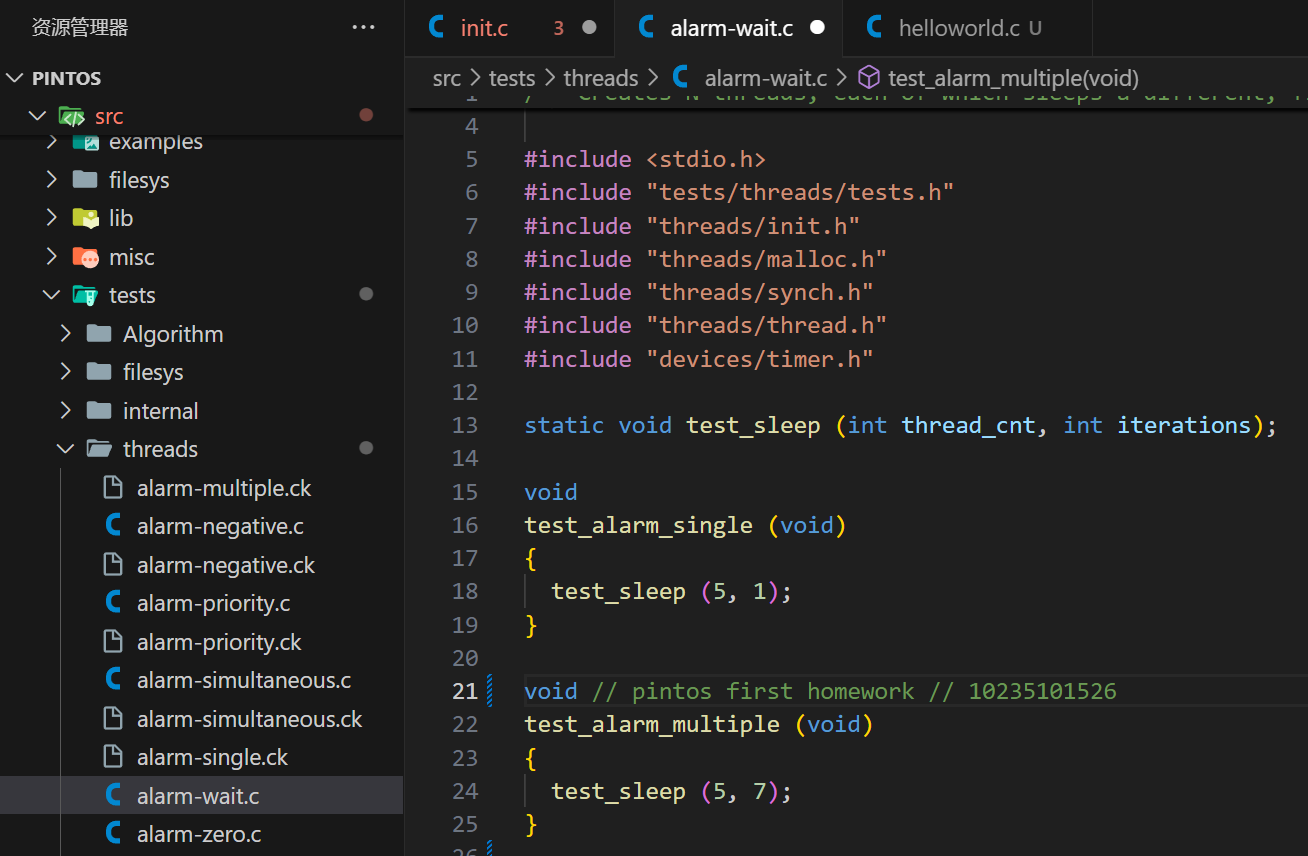
\includegraphics[width=0.5\textwidth]{img2/1.png}
  \caption{在VSCode中打开Pintos项目}
\end{figure}

作好注释,表示这是第二次课程的作业,记录学号以确保本截图来自本人。

\subsection{添加指定内容}

进入src/test/threads/test.c与test.h,新增hello-world部分的代码。

\begin{figure}[H]
  \centering
  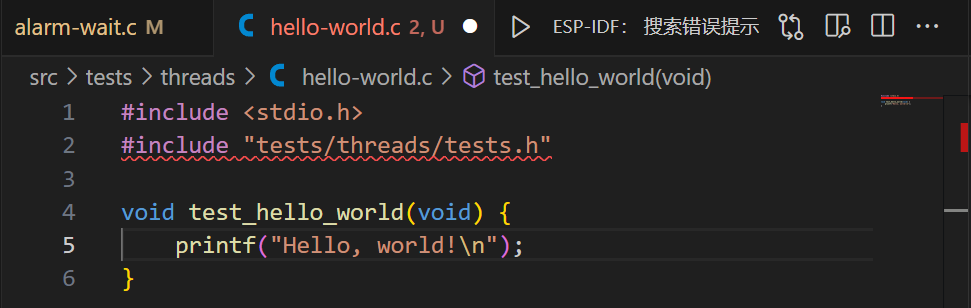
\includegraphics[width=0.5\textwidth]{img2/helloworld.png}
  \caption{在VSCode中添加hello-world.c代码}
\end{figure}

\begin{figure} [H]
  \centering
  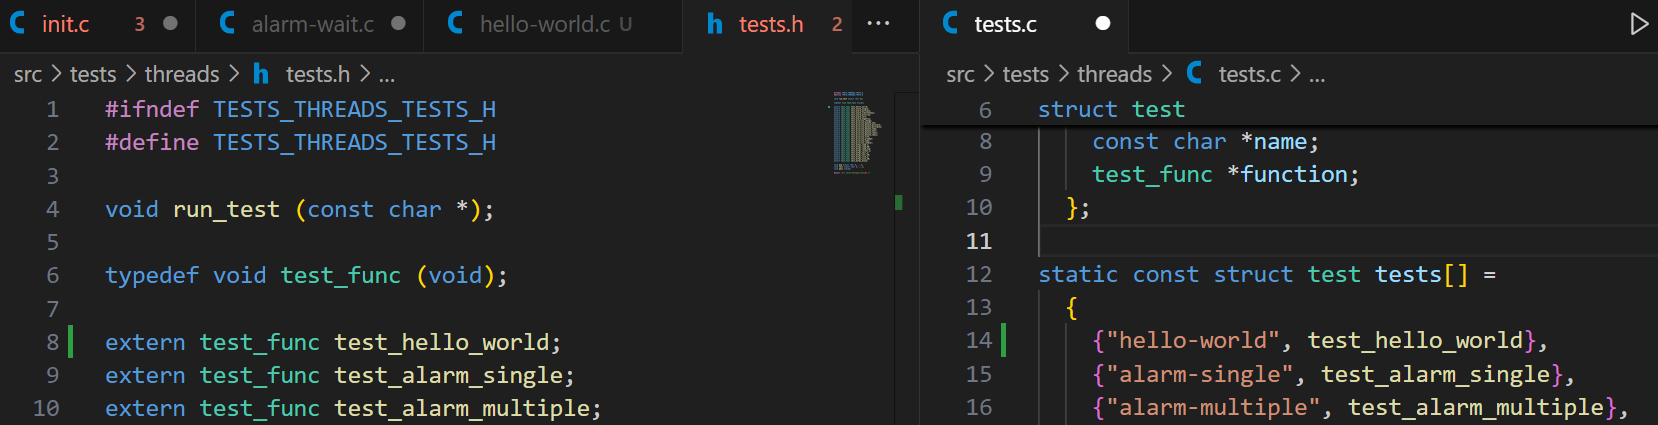
\includegraphics[width=0.5\textwidth]{img2/2.png}
  \caption{添加指定内容}
\end{figure}

\subsection{全局搜索,查看编译方式}

使用 Ctrl + Shift + F 进行全局搜索,因为我们要通过一个测试,
而之前我们已经通过了alarm-multiple的测试,所以不妨使用全局搜索查看它是怎样运行的。

\begin{figure}[H]
  \centering
  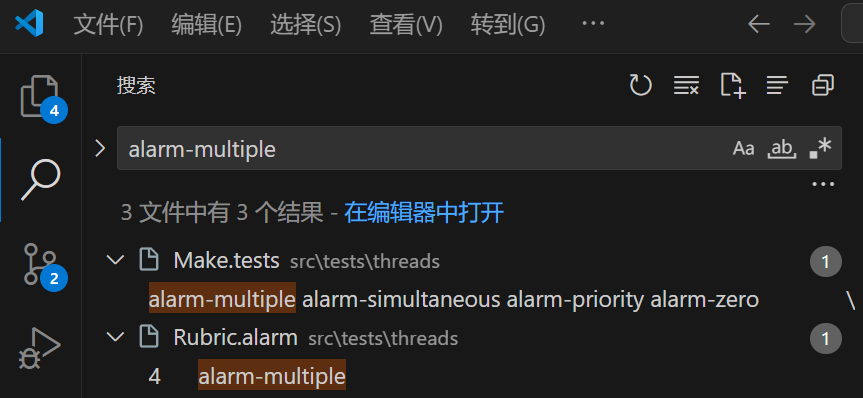
\includegraphics[width=0.5\textwidth]{img2/3.png}
  \caption{全局搜索,查看编译方式}
\end{figure}

可以看到,有三个结果,其中一个是我们已经操作过的test.c中的内容,接下来,我们应该对Make.testc文件进行重点关注。

我们增加一个名为"hello-world"的测试,反斜杠代表不换行。

\begin{figure}[H]
  \centering
  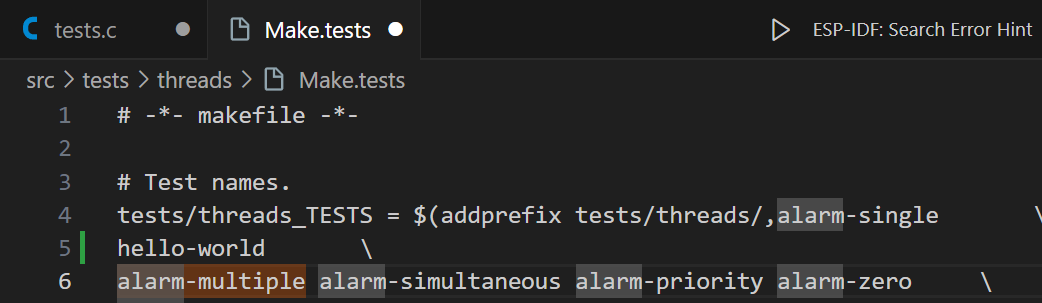
\includegraphics[width=0.5\textwidth]{img2/4.png}
  \caption{Make.testc文件}
\end{figure}

在下面的thread-SRC 中按照相关的格式添加hello-world部分的代码。

\begin{figure}[H]
  \centering
  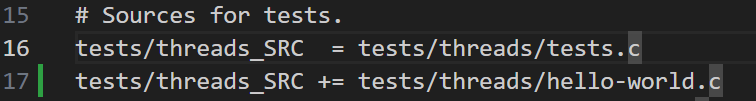
\includegraphics[width=0.5\textwidth]{img2/5.png}
  \caption{Make.testc文件}
\end{figure}

\subsection{尝试运行}

接下来,保存,尝试运行。

\begin{figure}[H]
  \centering
  
\includegraphics[width=0.5\textwidth]{img2/6.png}
  \caption{尝试运行}
\end{figure}

运行命令:\textbf{pintos -- -q run hello-world},结果如下所示:

\begin{figure}[H]
  \centering
  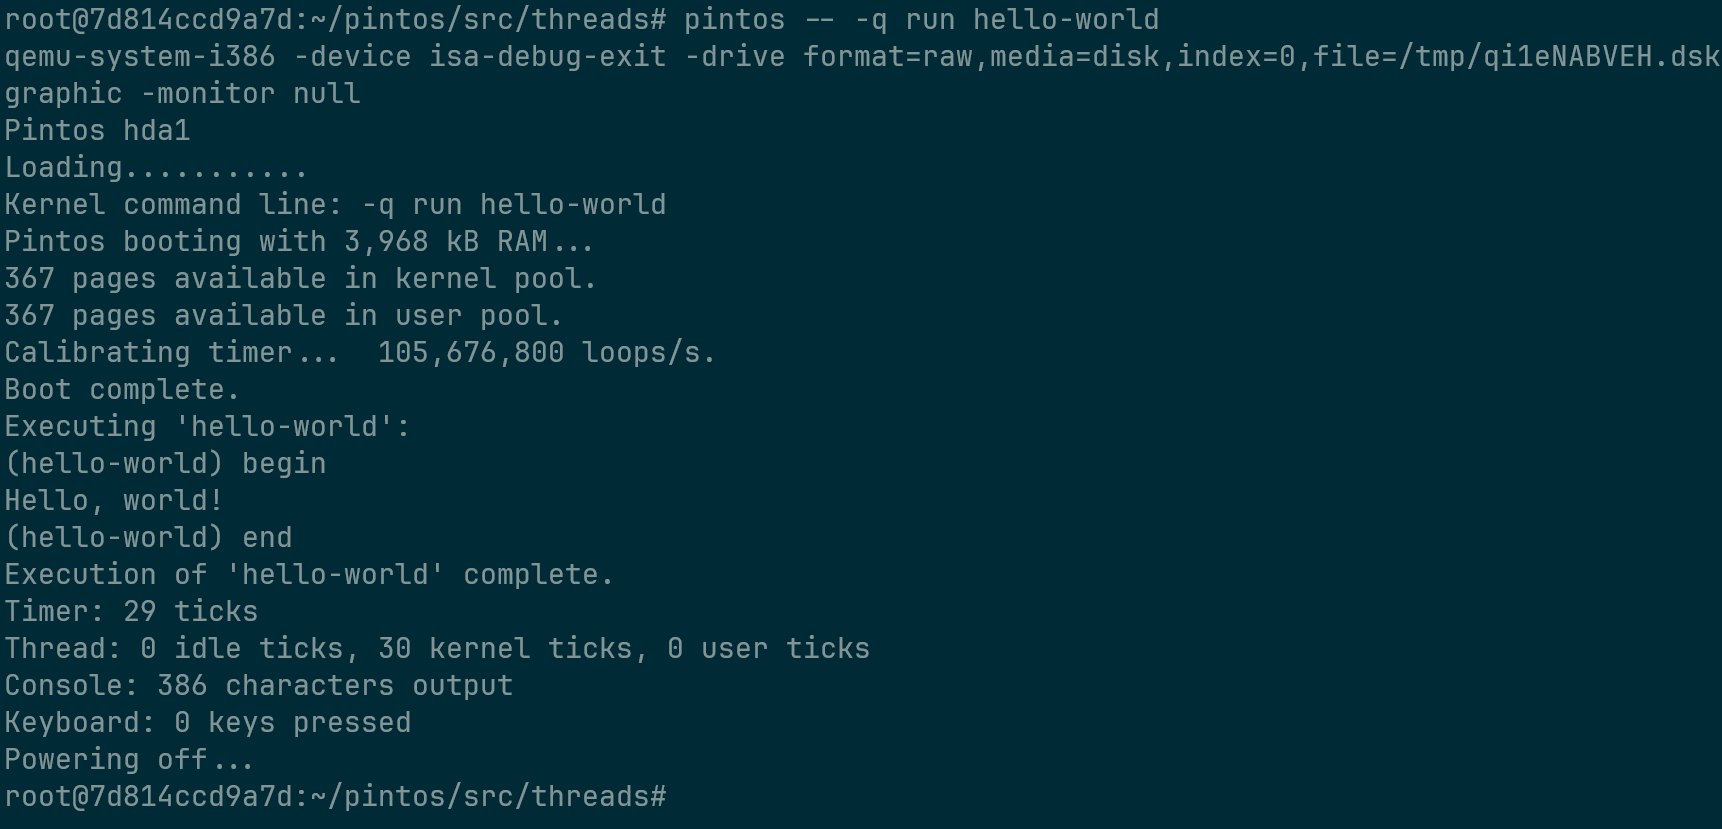
\includegraphics[width=0.5\textwidth]{img2/success.png}
  \caption{运行结果}
\end{figure}

\subsection{配置make check}

pintos的测试检查使用perl脚本语言,观察其他的.ck文件,可以发现格式几乎一致。
不同的地方在于预期的结果不同。

故根据其他两个文件对比,可以照搬格式,然后将输出结果写入特殊的位置即可。

注意到其他文件里最后都留了一行空行,我们也可以留以避免不必要的BUG。

\begin{figure}[H]
  \centering
  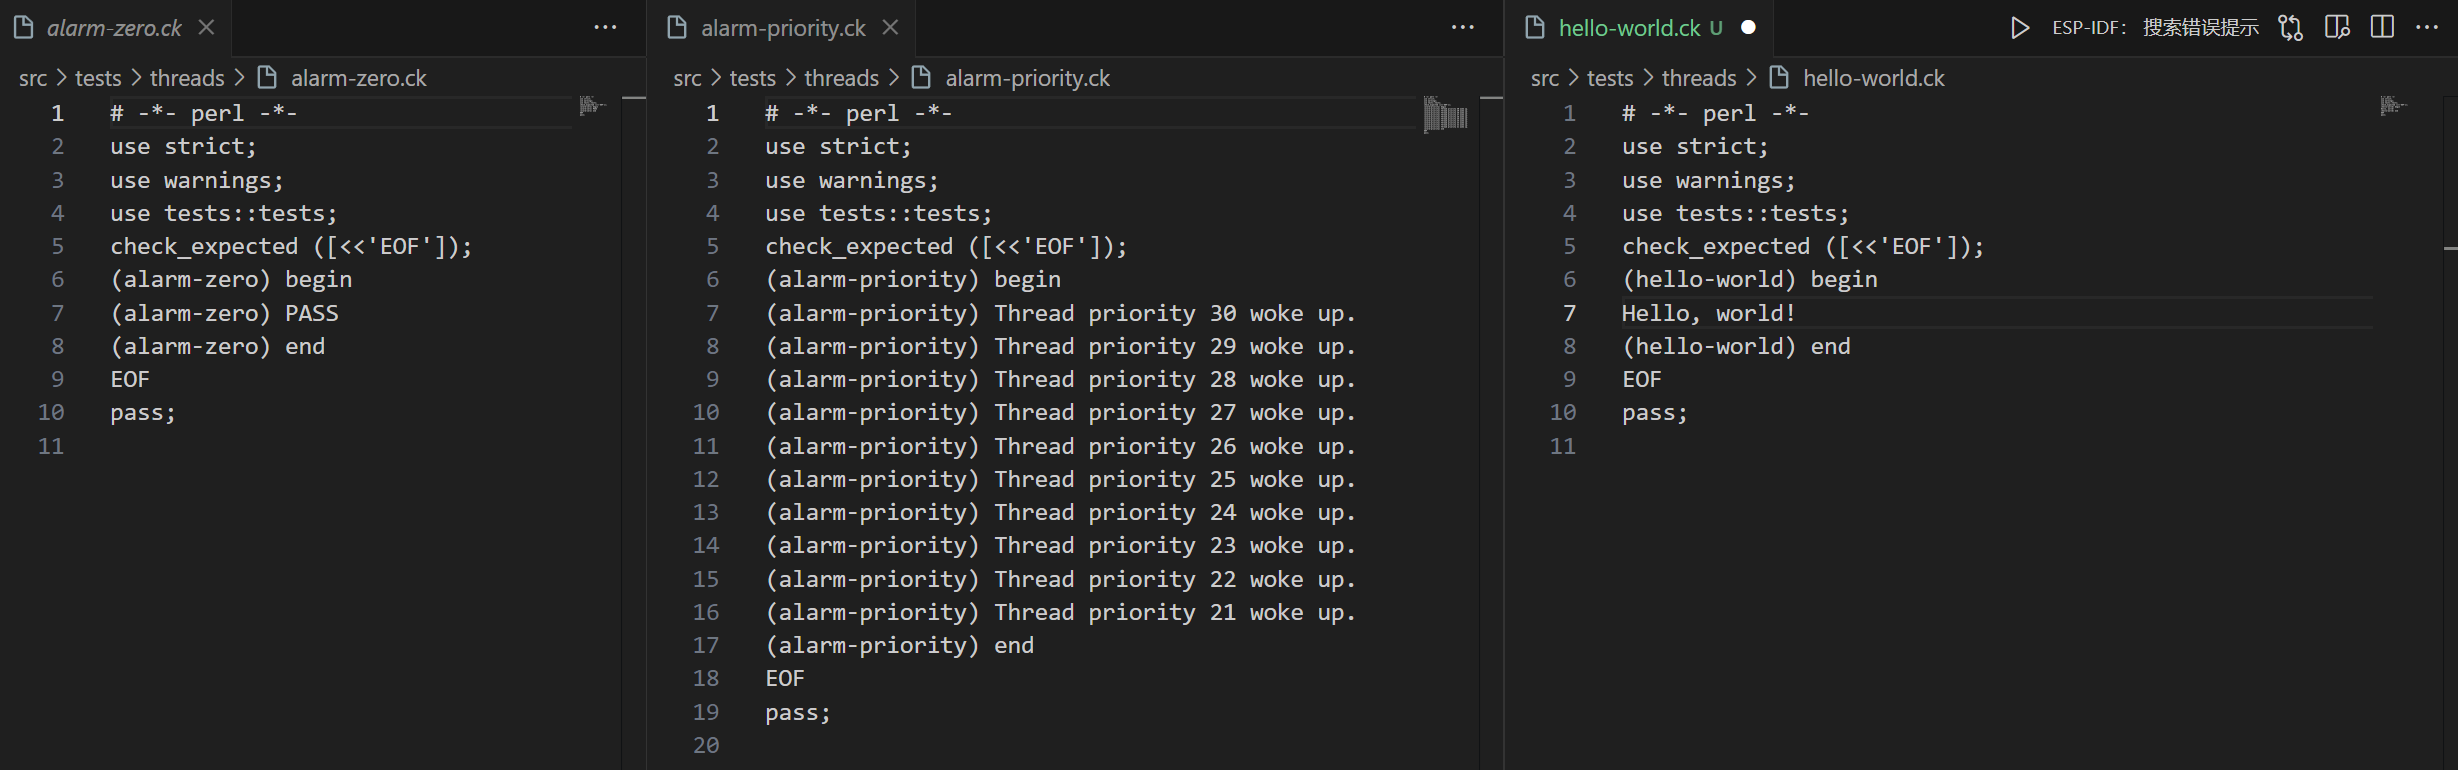
\includegraphics[width=0.5\textwidth]{img2/final.png}
  \caption{配置make check}
\end{figure}

保存文件,并查看make check指令的结果,如下图所示:

\begin{figure}{H}
  \centering
  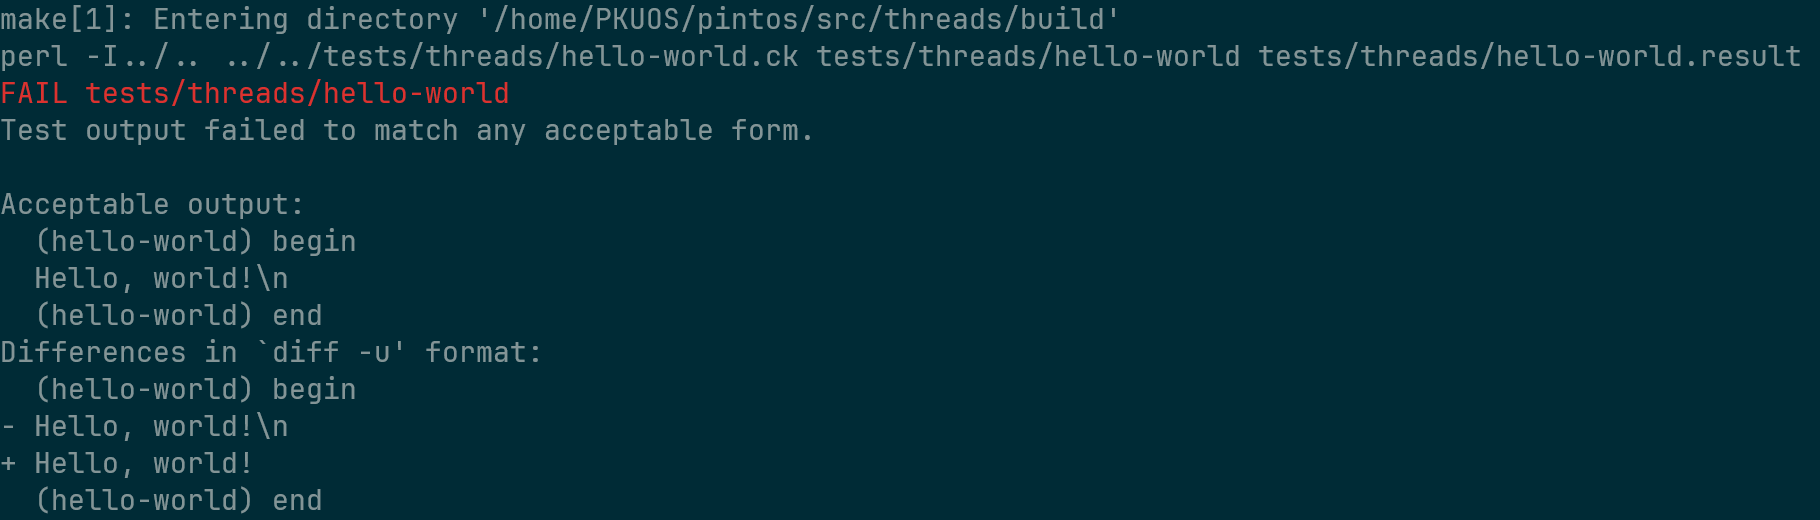
\includegraphics[width=0.5\textwidth]{img2/fault.png}
  \caption{Make Check 结果}
\end{figure}

发现结果错误,猜测应该是由于\textbackslash n 导致的,换行符的存在可能会对缓冲区造成一定的影响。

故去掉换行符,修改如下:

\begin{figure} [H]
  \centering
  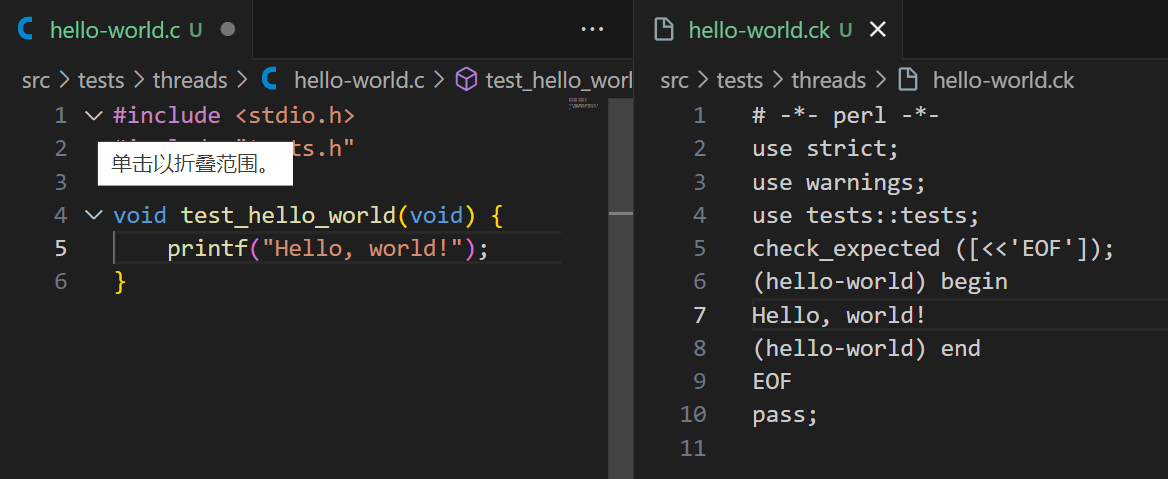
\includegraphics[width=0.5\textwidth]{img2/change.png}
  \caption{修改换行符}
\end{figure}

修改结束后再次执行\texttt{make check}指令,通过测试点。

\begin{figure}[H]
  \centering
  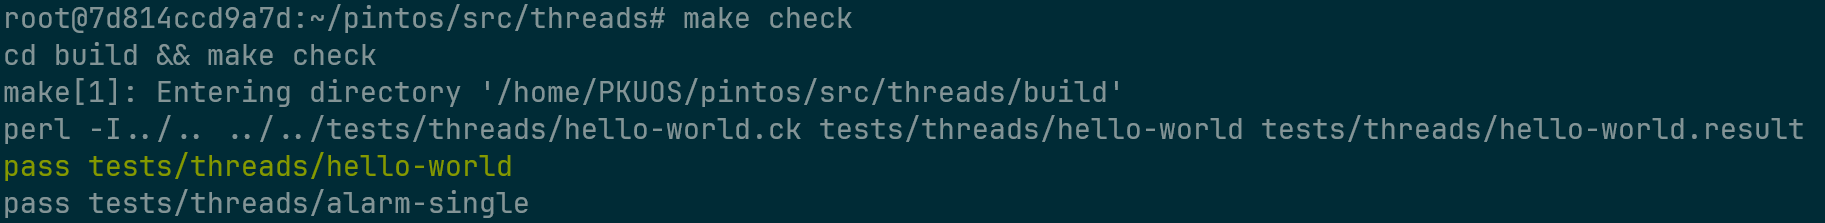
\includegraphics[width=0.5\textwidth]{img2/success2.png}
  \caption{Make Check 结果}
\end{figure}

\subsection{实验总结}

通过本次实验,我成功地在Pintos系统中创建了一个新的测试用例 \texttt{hello-world},并了解了Pintos操作系统架构的部分实现细节。实验过程中,我掌握了以下关键知识点:

\begin{enumerate}
    \item \textbf{测试用例的创建与调试}:通过编写 \texttt{hello-world} 测试用例,我学习了Pintos测试框架的工作原理,理解了如何对操作系统的底层代码进行修改,并通过 \texttt{make check} 命令验证测试结果。
    
    \item \textbf{调试与问题分析}:实验中遇到了输出不符合预期的问题,最终通过分析测试输出格式,发现是由于缺少换行符导致的缓冲区问题。
    
    \item \textbf{实验工具的使用}:我还掌握了如何使用VSCode的Remote Development插件进行远程开发,以及如何通过全局搜索快速定位关键文件和代码模块,提升了代码调试和问题解决的效率。
\end{enumerate}

\section{附录}

本次实验作出修改的代码如下所示:

同时上传到了 Github 之上,仓库地址为:

\lstinputlisting[language = C , title = hello-world.c] {lst2/hello-world.c}

\lstinputlisting[language = C , title = hello-world.ck]{lst2/hello-world.ck}

\lstinputlisting[language = C , title = Make.tests]{lst2/Make.tests}

\end{document}